\documentclass[aspectratio=169]{beamer}

% ---------- Packages ----------
\usepackage[utf8]{inputenc}
\usepackage[T1]{fontenc}
\usepackage{textcomp}      % \textonehalf, \textonequarter
\usepackage{tikz}
\usetikzlibrary{arrows.meta,positioning,calc,shapes}
\usepackage{pgfplots}
\pgfplotsset{compat=1.17}

% ---------- Theme / chrome ----------
\usetheme{default}
\setbeamertemplate{navigation symbols}{}
\setbeamertemplate{headline}{}
\setbeamercolor{background canvas}{bg=white}

% ---------- Colors (sampled from the original deck) ----------
\definecolor{headerblue}{RGB}{16,57,69}
\definecolor{footerblue}{RGB}{157,195,231}
\definecolor{purplebox}{RGB}{16,57,69}
\definecolor{lavbg}{RGB}{180,200,239}
\definecolor{bitblue}{RGB}{186,212,236}
\definecolor{bitred}{RGB}{250,150,150}
\definecolor{plotred}{RGB}{250,0,10}
\definecolor{titletext}{RGB}{31,42,120}

\setbeamersize{text margin left=0.9cm,text margin right=0.9cm}

% ---------- Frame title = blue bar spanning full slide width ----------
\setbeamercolor{frametitle}{fg=white,bg=headerblue}
\setbeamerfont{frametitle}{size=\LARGE,series=\bfseries}
\makeatletter
\setbeamertemplate{frametitle}{
  \nointerlineskip
  \begin{beamercolorbox}[wd=\paperwidth,ht=1.15cm,dp=0.35cm,leftskip=0.5cm,colsep=0pt]{frametitle}
    \usebeamerfont{frametitle}\insertframetitle
  \end{beamercolorbox}
  \vspace{0.3cm}
}
\makeatother

% ---------- Footline = light-blue bar with speaker credit ----------
\setbeamercolor{footline}{fg=black,bg=footerblue}
\setbeamerfont{footline}{size=\normalsize}
\setbeamertemplate{footline}{
  \begin{beamercolorbox}[wd=\paperwidth,ht=0.5cm,dp=0.3cm,leftskip=0.4cm,colsep=0pt]{footline}
    \usebeamerfont{footline}Speaker: Sumaiya Sultana Labiba (2305044)
  \end{beamercolorbox}
}

% ---------- Placeholder box for images the original deck embedded ----------
% Usage: \personph{<node name>}{<x>}{<y>}{<filename label>}{<caption>}
\newcommand{\personph}[5]{%
  \node (#1) at (#2,#3)
        {\includegraphics[width=1.3cm,height=1.5cm,keepaspectratio]{#4}};%
  \node[font=\normalsize] at (#2,#3-1.0) {#5};%
}


\title{Quantum Cryptography: Part 3 -- Eve, Detection \& Future}
\author{Sumaiya Sultana Labiba (2305044)}

\begin{document}

% ============================================================
% Slide 1 (title slide)
% ============================================================
\begin{frame}{Quantum Cryptography : Part 3}
\vspace{1.3cm}
\begin{center}
{\usebeamerfont{frametitle}\color{titletext}\Huge Eve, Detection \& Future}\\[1.1cm]
{\Large ``The attacker becomes part of the experiment.''}
\end{center}
\end{frame}

% ============================================================
% Slides 2-5: Eve Enters the Channel  (4 build steps)
% ============================================================
\begin{frame}{Eve Enters the Channel}
\begin{center}
\begin{tikzpicture}
  \node<4->[red,font=\small] at (4,2.1) {intercepts \& measures};

  \personph{alice}{0}{0.8}{alice.png}{Alice}
  \personph{bob}{8}{0.8}{bob.png}{Bob}

  % Step 1 only: single direct channel
  \draw<1>[-{Latex[length=3mm]},thick] (alice) -- (bob)
       node[midway,above,font=\small]{Quantum Channel};

  % Step 2 onward: Eve inserted, channel splits in two
  \onslide<2->{
  \personph{eve}{4}{0.8}{eve.png}{Eve}
  }
  \node<2->[font=\normalsize] at (4,-0.2) {Eve};
  \draw<2->[-{Latex[length=3mm]},thick] (alice) -- (eve)
       node[midway,above,font=\small]{Quantum Channel};
  \draw<2->[-{Latex[length=3mm]},thick] (eve) -- (bob)
       node[midway,above,font=\small]{Quantum Channel};
\end{tikzpicture}
\end{center}
\vspace{0.2cm}
\begin{center}
\only<3->{Eve sits in the path, wanting the key --- with one option: measure it}
\end{center}
\end{frame}

% ============================================================
% Slides 6-9: Intercept-Measure-Resend  (4 build steps)
% ============================================================
\begin{frame}{Intercept-Measure-Resend}
\begin{center}
\begin{tikzpicture}
  \node<3->[red,font=\small] at (4,2.8) {measures in wrong basis(guessed!)};

  \personph{alice}{0}{0.8}{alice.png}{Alice}
  \personph{eve}{4}{0.8}{eve.png}{Eve}
  \node[font=\normalsize] at (4,-0.2) {Eve};
  \personph{bob}{8}{0.8}{bob.png}{Bob}

  \draw[-{Latex[length=3mm]},thick] (alice) -- (eve)
       node[midway,above,font=\small]{Photon $\psi$};
  \draw<4->[-{Latex[length=3mm]},thick,red] (eve) -- (bob)
       node[midway,above,font=\small,text=red]{Disturbed $\psi^{*}$};

  \draw<1>[red,line width=2pt] (alice) ellipse (1.05cm and 1.3cm);
  \draw<2->[red,line width=2pt] (eve) ellipse (1.05cm and 1.3cm);
\end{tikzpicture}
\end{center}
\vspace{0.1cm}
\begin{center}
\only<1>{A photon leaves Alice, encoded in her random basis.}%
\only<2>{Eve intercepts it mid-flight}%
\only<3>{She must guess the basis --- half the time, she's wrong.}%
\only<4>{Wrong guess = altered state sent to Bob. The evidence just changed.}
\end{center}
\end{frame}

% ============================================================
% Slides 10-15: Why Errors Appear  (6 build steps)
% ============================================================
\begin{frame}{Why Errors Appear}
\begin{itemize}
  \item<1-> Eve guesses the \textcolor{red}{correct} basis $\Rightarrow$ no disturbance, no evidence.
  \item<2-> Eve guesses the \textcolor{red}{wrong} basis $\Rightarrow$ Bob's result becomes random
  \item<3-> Probability of a wrong guess: \textonehalf
  \item<4-> Given a wrong guess, probability Bob's bit flips: \textonehalf
\end{itemize}
\vspace{0.35cm}
\onslide<5->{%
\begin{center}
\begin{minipage}{9.3cm}
\colorbox{headerblue}{\parbox{9.3cm}{\centering\color{white}\vspace{3pt}Net error introduced by Eve:\vspace{3pt}}}\\[-0.4pt]
\colorbox{lavbg}{\parbox{9.3cm}{\centering\vspace{5pt}\Large\textonehalf $\times$ \textonehalf\ = \textonequarter\ = 25\%\vspace{5pt}}}
\end{minipage}
\end{center}}
\vspace{0.25cm}
\onslide<6->{\begin{center}\color{red} That's not a bug --- that's her fingerprint.\end{center}}
\end{frame}

% ============================================================
% Slides 16-18: Catching Eve: Sampling the Key (3 build steps)
% ============================================================
\begin{frame}{Catching Eve: Sampling the Key}
\begin{center}
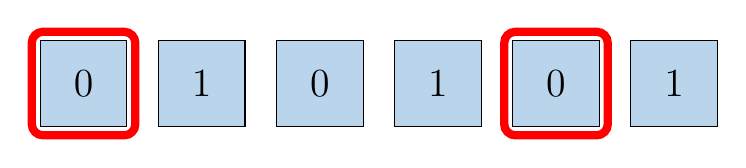
\begin{tikzpicture}[bit/.style={draw,fill=bitblue,minimum width=1.1cm,minimum height=1.1cm,font=\Large}]
  \node[bit] (b1) at (1.5,0) {0};
  \node[bit] (b2) at (3.0,0) {1};
  \node[bit] (b3) at (4.5,0) {0};
  \node[bit] (b4) at (6.0,0) {1};
  \node[bit] (b5) at (7.5,0) {0};
  \node[bit] (b6) at (9.0,0) {1};
  \draw<2->[red,line width=3pt,rounded corners] ($(b1.north west)+(-0.1,0.1)$) rectangle ($(b1.south east)+(0.1,-0.1)$);
  \draw<2->[red,line width=3pt,rounded corners] ($(b5.north west)+(-0.1,0.1)$) rectangle ($(b5.south east)+(0.1,-0.1)$);
\end{tikzpicture}
\end{center}
\vspace{0.3cm}
\begin{center}
\only<1>{A small random sample of the sifted key is picked.}%
\only<2->{sacrificed publicly to check for tampering}
\end{center}
\onslide<3->{\begin{center}\color{blue} If nobody touched the channel, these should match exactly.\end{center}}
\end{frame}

% ============================================================
% Slide 19: The Error Rate Tells the Story
% ============================================================
\begin{frame}{The Error Rate Tells the Story}
\begin{center}
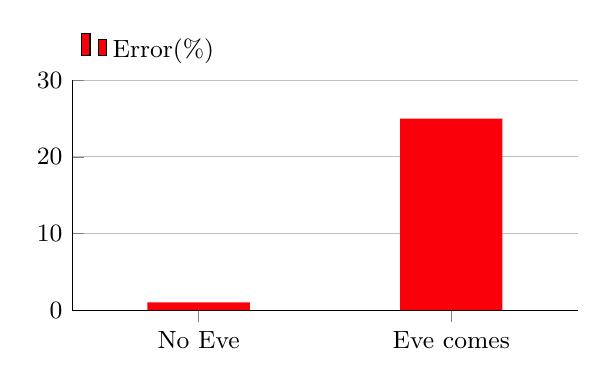
\begin{tikzpicture}
\begin{axis}[
  ybar, bar width=1.3cm,
  width=8.0cm,height=4.5cm,
  ymin=0,ymax=30,
  symbolic x coords={No Eve,Eve comes},
  xtick=data,
  tick label style={font=\small},
  legend style={at={(0,1.03)},anchor=south west,draw=none,font=\small},
  ymajorgrids,
  axis lines*=left,
  enlarge x limits=0.5,
]
\addplot[fill=plotred,draw=none] coordinates {(No Eve,1.0) (Eve comes,25.0)};
\addlegendentry{Error(\%)}
\end{axis}
\end{tikzpicture}
\end{center}
\begin{center}
Near zero without an eavesdropper --- a clear jump to $\sim$25\% with one. Unmissable.
\end{center}
\end{frame}

% ============================================================
% Slides 20-21: Bit-by-Bit: Where They Disagree (2 build steps)
% ============================================================
\begin{frame}{Bit-by-Bit: Where They Disagree}
\begin{center}
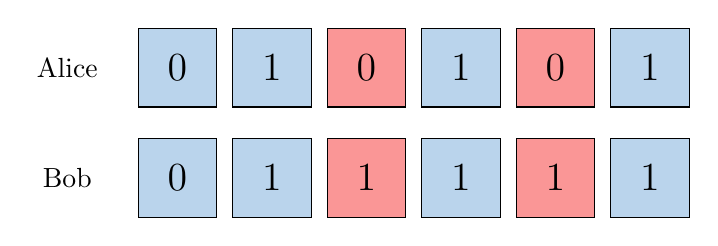
\begin{tikzpicture}[
  bit/.style={draw,minimum width=1.0cm,minimum height=1.0cm,font=\Large}
]
  \node at (-1.0,0.7) {Alice};
  \node[bit,fill=bitblue] (a1) at (0.4,0.7) {0};
  \node[bit,fill=bitblue] (a2) at (1.6,0.7) {1};
  \node<1>[bit,fill=bitblue] (a3) at (2.8,0.7) {0};
  \node<2>[bit,fill=bitred]  (a3) at (2.8,0.7) {0};
  \node[bit,fill=bitblue] (a4) at (4.0,0.7) {1};
  \node<1>[bit,fill=bitblue] (a5) at (5.2,0.7) {0};
  \node<2>[bit,fill=bitred]  (a5) at (5.2,0.7) {0};
  \node[bit,fill=bitblue] (a6) at (6.4,0.7) {1};

  \node at (-1.0,-0.7) {Bob};
  \node[bit,fill=bitblue] (b1) at (0.4,-0.7) {0};
  \node[bit,fill=bitblue] (b2) at (1.6,-0.7) {1};
  \node<1>[bit,fill=bitblue] (b3) at (2.8,-0.7) {1};
  \node<2>[bit,fill=bitred]  (b3) at (2.8,-0.7) {1};
  \node[bit,fill=bitblue] (b4) at (4.0,-0.7) {1};
  \node<1>[bit,fill=bitblue] (b5) at (5.2,-0.7) {1};
  \node<2>[bit,fill=bitred]  (b5) at (5.2,-0.7) {1};
  \node[bit,fill=bitblue] (b6) at (6.4,-0.7) {1};
\end{tikzpicture}
\end{center} 
\vspace{0.3cm}
\begin{center}
\only<1>{Compare Alice's and Bob's sampled bits directly.}%
\only<2>{Every mismatch is Eve's signature --- written in physics.}
\end{center}
\end{frame}


% ============================================================
% Slide 22: Classical vs. Quantum Eavesdropping
% ============================================================
\begin{frame}{Classical vs. Quantum Eavesdropping}
\begin{center}
\begin{columns}[T]
\begin{column}{0.46\textwidth}
\colorbox{purplebox}{\parbox{\linewidth}{\centering\color{white}\Large\vspace{4pt}Classical\vspace{4pt}}}\\[-0.4pt]
\colorbox{lavbg}{\parbox{\linewidth}{\vspace{5pt}
\begin{minipage}[t][1.75cm][t]{\linewidth}
\begin{itemize}
  \item Tap a wire, copy the signal
  \item The original is untouched
  \item No trace left behind
\end{itemize}
\end{minipage}
\vspace{2pt}}}
\end{column}
\begin{column}{0.46\textwidth}
\colorbox{purplebox}{\parbox{\linewidth}{\centering\color{white}\Large\vspace{4pt}Quantum\vspace{4pt}}}\\[-0.4pt]
\colorbox{lavbg}{\parbox{\linewidth}{\vspace{5pt}
\begin{itemize}
  \item Measuring changes state
  \item Original is disturbed
  \item Detected, every time
\end{itemize}
\vspace{2pt}}}
\end{column}
\end{columns}
\end{center}
\vspace{0.5cm}
\begin{center}
Eavesdropping stops being invisible --- it becomes measurable.
\end{center}
\end{frame}

% ============================================================
% Slides 23-25: Detection (3 build steps)
% ============================================================
\begin{frame}{Detection}
\vspace{0.8cm}
\begin{center}
\only<1>{\Large Comparing the sampled bits\ldots}%
\only<2->{\textbf{\color{red}\huge EVE DETECTED!!!}}
\end{center}
\onslide<3->{%
\vspace{0.6cm}
\begin{center}
Not suspected. Not guessed.\\
Detected --- by the laws of physics.
\end{center}}
\end{frame}

% ============================================================
% Slides 26-30: Beyond the Lab (5 build steps)
% ============================================================
\begin{frame}{Beyond the Lab}
\begin{itemize}
  \item<1-> Already running in real fiber-optic QKD networks
  \item<2-> Deployed via satellite --- e.g. China's Micius
  \item<3-> Seed of a quantum internet: security built into physics itself
\end{itemize}
\vspace{0.4cm}
\onslide<4->{\begin{center}\color{red} ``What if looking at a secret could change it?''\end{center}}
\vspace{0.15cm}
\onslide<5->{\begin{center}\color{blue}\small Now you know: it does. And that's what makes it unbreakable.\end{center}}
\end{frame}

% ============================================================
% Slide 31: Thank You
% ============================================================
\begin{frame}{Quantum Cryptography : Part 3}
\vspace{0cm}
\begin{center}
{\usebeamerfont{frametitle}\color{titletext}\Huge Thank You!}
\end{center}
\end{frame}

\end{document}

